\section{Исследовательская часть}

\subsection{Технические характеристики}
Технические характеристики устройства, на котором выполнялось тестирование, следующие:
\begin{itemize}
    \item Операционная система: Windows 10 64-bit;
    \item Память 8 ГБ;
    \item Процессор: Intel(R) Core(TM) i7-8550U CPU @ 1.80GHz   1.99 GHz.
\end{itemize}

\subsection{Демонстрация работы программы}
На рисунке \ref{fig:program} представлен результат работы программы.

\begin{figure}[H]
\center{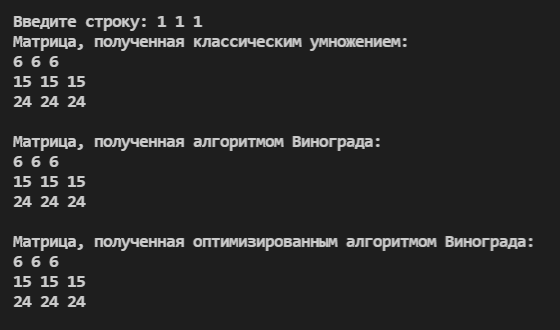
\includegraphics[scale=0.9]{pictures/program.png}}
\caption{Результат работы программы.}
\label{fig:program}
\end{figure}

\newpage
\subsection{Время работы алгоритмов}

Бал проведён замер времени работы из алгоритмов. Каждый замер времени проводился 10 раз и результат усреднялся. Первый эксперимент производится для лучшего случая на матрицах размерами от 100 на 100 до 500 на 500 с шагом 100. Рисунок \ref{fig:t_even}.

\begin{figure}[H]
\center{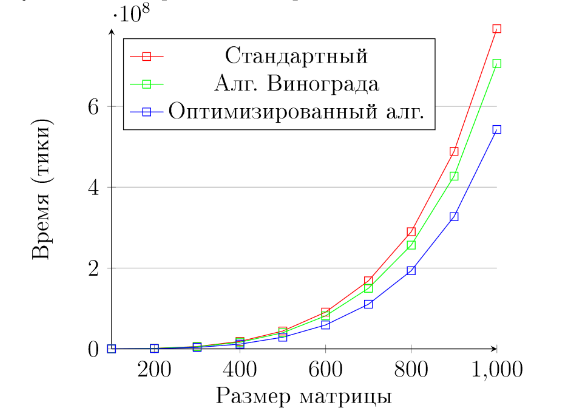
\includegraphics[scale=0.7]{pictures/lag1.png}}
\caption{Замеры времени на чётном количестве строк и столбцов квадратных матриц.}
\label{fig:t_even}
\end{figure}

Второй эксперимент производится для худшего случая, когда заданы матрицы с нечётными размерами от 101 на 101 до 501 на 501 с шагом 100. Рисунок \ref{fig:t}.

\begin{figure}[H]
\center{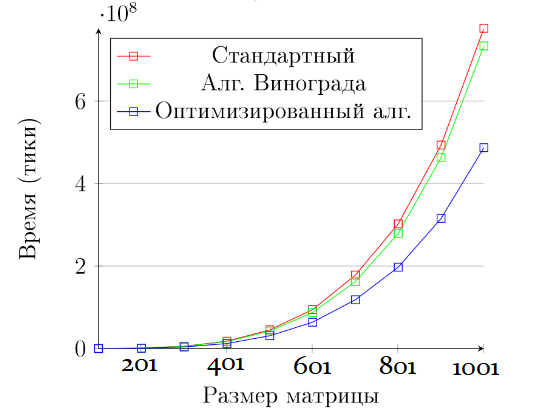
\includegraphics[scale=0.7]{pictures/alg2.png}}
\caption{Замеры времени на нечётном количестве строк и столбцов квадратных матриц.}
\label{fig:t}
\end{figure}

По результатам тестирования, все рассматриваемые алгоритмы реализованы правильно. Самым медленным оказался алгоритм классического умножения матриц, самым быстрым - оптимизированный алгоритм Винограда.

\subsection{Вывод}
В данном разделе протестированы алгоритмы умножения матриц. Классический алгоритм показал худшие результаты, что и следовало ожидать. Оптимизированный алгоритм Винограда проявил себя лучше остальных. Экспериментально было подтверждено различие по временной эффективности алгоритмов умножения матриц на материале замеров процессорного времени выполнения реализации на варьирующихся размерах матриц. Так, самым быстрым является оптимизированный алгоритм Винограда, на размере матрицы 400 на 400 он работает в 1,3 раза быстрее алгоритма Винограда без оптимизации и в 1,23 раз быстрее классического алгоритма умножения. Алгоритмы Винограда и классического умножения примерно сопоставимы.